\chapter{Design}
In this chapter we focus on how to implement what we have specified in the analysis chapter.
First, we describe our application's architecture.
Then, we discuss what technologies were considered for implementing the application, and which of the technologies were chosen and why.
We name our application "Choose well".

\section{Architecture}
We design our solution\footnote{From now on we will be referring to our application as the solution as not to  confuse it with the actual applications which it consists of.  \label{fnlabel}} as multiple independent single-page web applications.
This decision is made to achieve better modularity. 
One of the applications is the guest dietary profile editor.
It allows a guest to set their dietary preferences like being allergic to something or being vegetarian.
Another application is the restaurant menu maker.
It serves for restaurant employees to specify their menu's contents.
Last application is the personalized menu viewer for restaurant guests.
It combines information gathered by the other applications to display personalized menus to guests. 
% \todo[inline]{Later - add figure number}
Figure x contains a depiction of our solution's architecture.

\begin{figure}[h]
  \centering
  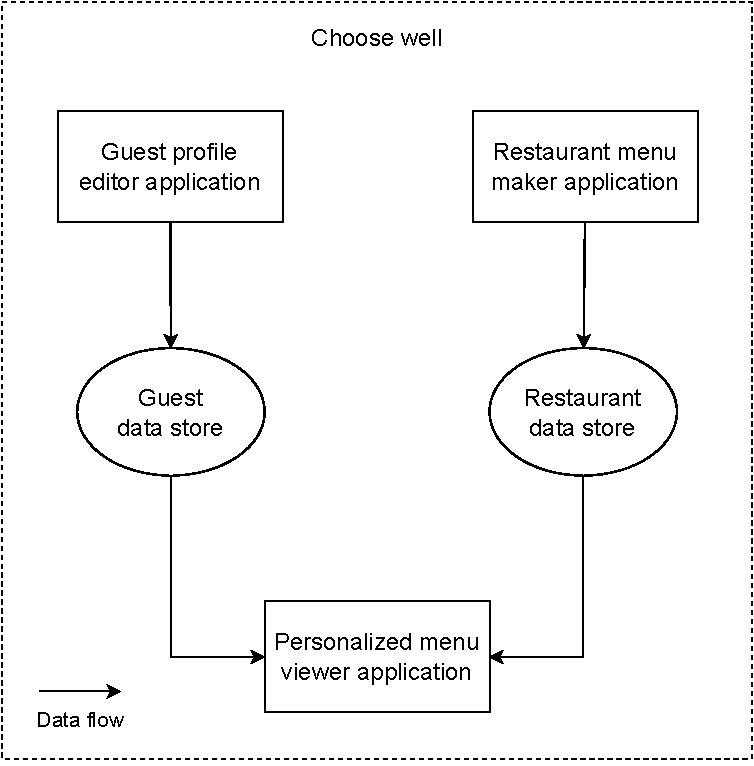
\includegraphics[width=0.75\linewidth]{master-thesis/img/architecture_data_flow.pdf}
  \caption{The solution's architecture}
\end{figure}

\section{Technological stack}
This section contains an overview of considered tools for implementing our solution.
We also note which technologies we choose and why.

\subsection*{User interface}
We choose \textbf{React}\footnote{\url{https://react.dev}  \label{fnlabel}} for developing the UI of the applications.
This decision is being made on the account that Solid for the client side is programmed for React.

\subsection*{Programming language}
As for a programming language, JavaScript and TypeScript were considered.
Both languages are supported by React, and we chose \textbf{Typescript}\footnote{\url{https://www.typescriptlang.org/docs}  \label{fnlabel}} because it adds type control to the programmer's code which makes it less error-prone.

% \todo[inline]{After exams - find a better reason why we choose Vite}
\subsection*{Build tool}
For the initial creation and building of applications during development, Create React App and Vite were considered.
We decided to choose \textbf{Vite}\footnote{\url{https://vitejs.dev/guide}  \label{fnlabel}} as it was recommended\footnote{\url{https://forum.solidproject.org/t/solid-app-development-tech-tools-stack-recommentation/5838/3}} by a developer who has been a member of the team which developed Solid.

\subsection*{Versioning}
We choose \textbf{Git}\footnote{\url{https://git-scm.com/docs}  \label{fnlabel}} to be able to have control over the versions of the applications as it is a very common option for a lot of projects.

\subsection*{Deployment}
Applications are hosted via \textbf{GitHub Pages}\footnote{\url{https://docs.github.com/en/pages}  \label{fnlabel}}.
We choose this technology as it is convenient

\subsection*{Package manager}
The \textbf{npm}\footnote{\url{https://docs.npmjs.com} \label{fnlabel}} package manager is used for handling packages in our projects.
We choose this technology because as is widely used and provides us with what we need for handling dependencies in the applications.

\subsection*{Responsive design}
Two options were considered in this topic: Bootstrap and Material UI.
Both of the technologies allow for mobile-first development approach.
We opted for \textbf{Bootstrap}\footnote{\url{https://getbootstrap.com} \label{fnlabel}} as it is easy to use and is well documented.

\subsection*{Persistence}
We can choose a traditional method for storing data, e.g. on our own server or in a cloud.
If we want to support the idea of decentralizing the web, we need to use a technology which enables us to shift the ownership of data to our users.
We want to use the \textbf{Solid}\footnote{\url{https://solidproject.org}  \label{fnlabel}} technology as it provides us with a way to store data in a decentralized manner.

\subsection*{Documentation}
The programmer documentation is written in markdown and is stored in the applications' public repositories\footnote{\url{https://github.com/JiriResler/solid-dietary-profile-editor}  \label{fnlabel}}\footnote{\url{https://github.com/JiriResler/solid-restaurant-guest-menu-viewer}  \label{fnlabel}}\footnote{\url{https://github.com/JiriResler/solid-restaurant-menu-editor}  \label{fnlabel}}.
The user documentation has a form of a webpage\footnote{\url{https://jiriresler.github.io/choose-well-website/index.html}  \label{fnlabel}} which is hosted on \textbf{GitHub Pages}.

\subsection*{Authentication}
The Inrupt's \textbf{solid-client}\footnote{\url{https://docs.inrupt.com/developer-tools/api/javascript/solid-client} \label{fnlabel}} JavaScript library for can be used for authentication of users.
We use the Inrupt's Solid React SDK\footnote{\url{https://docs.inrupt.com/developer-tools/javascript/react-sdk} \label{fnlabel}} which contains a Login component which uses the aforementioned library implicitly.